\begin{figure}[!htbp]
    \centering
    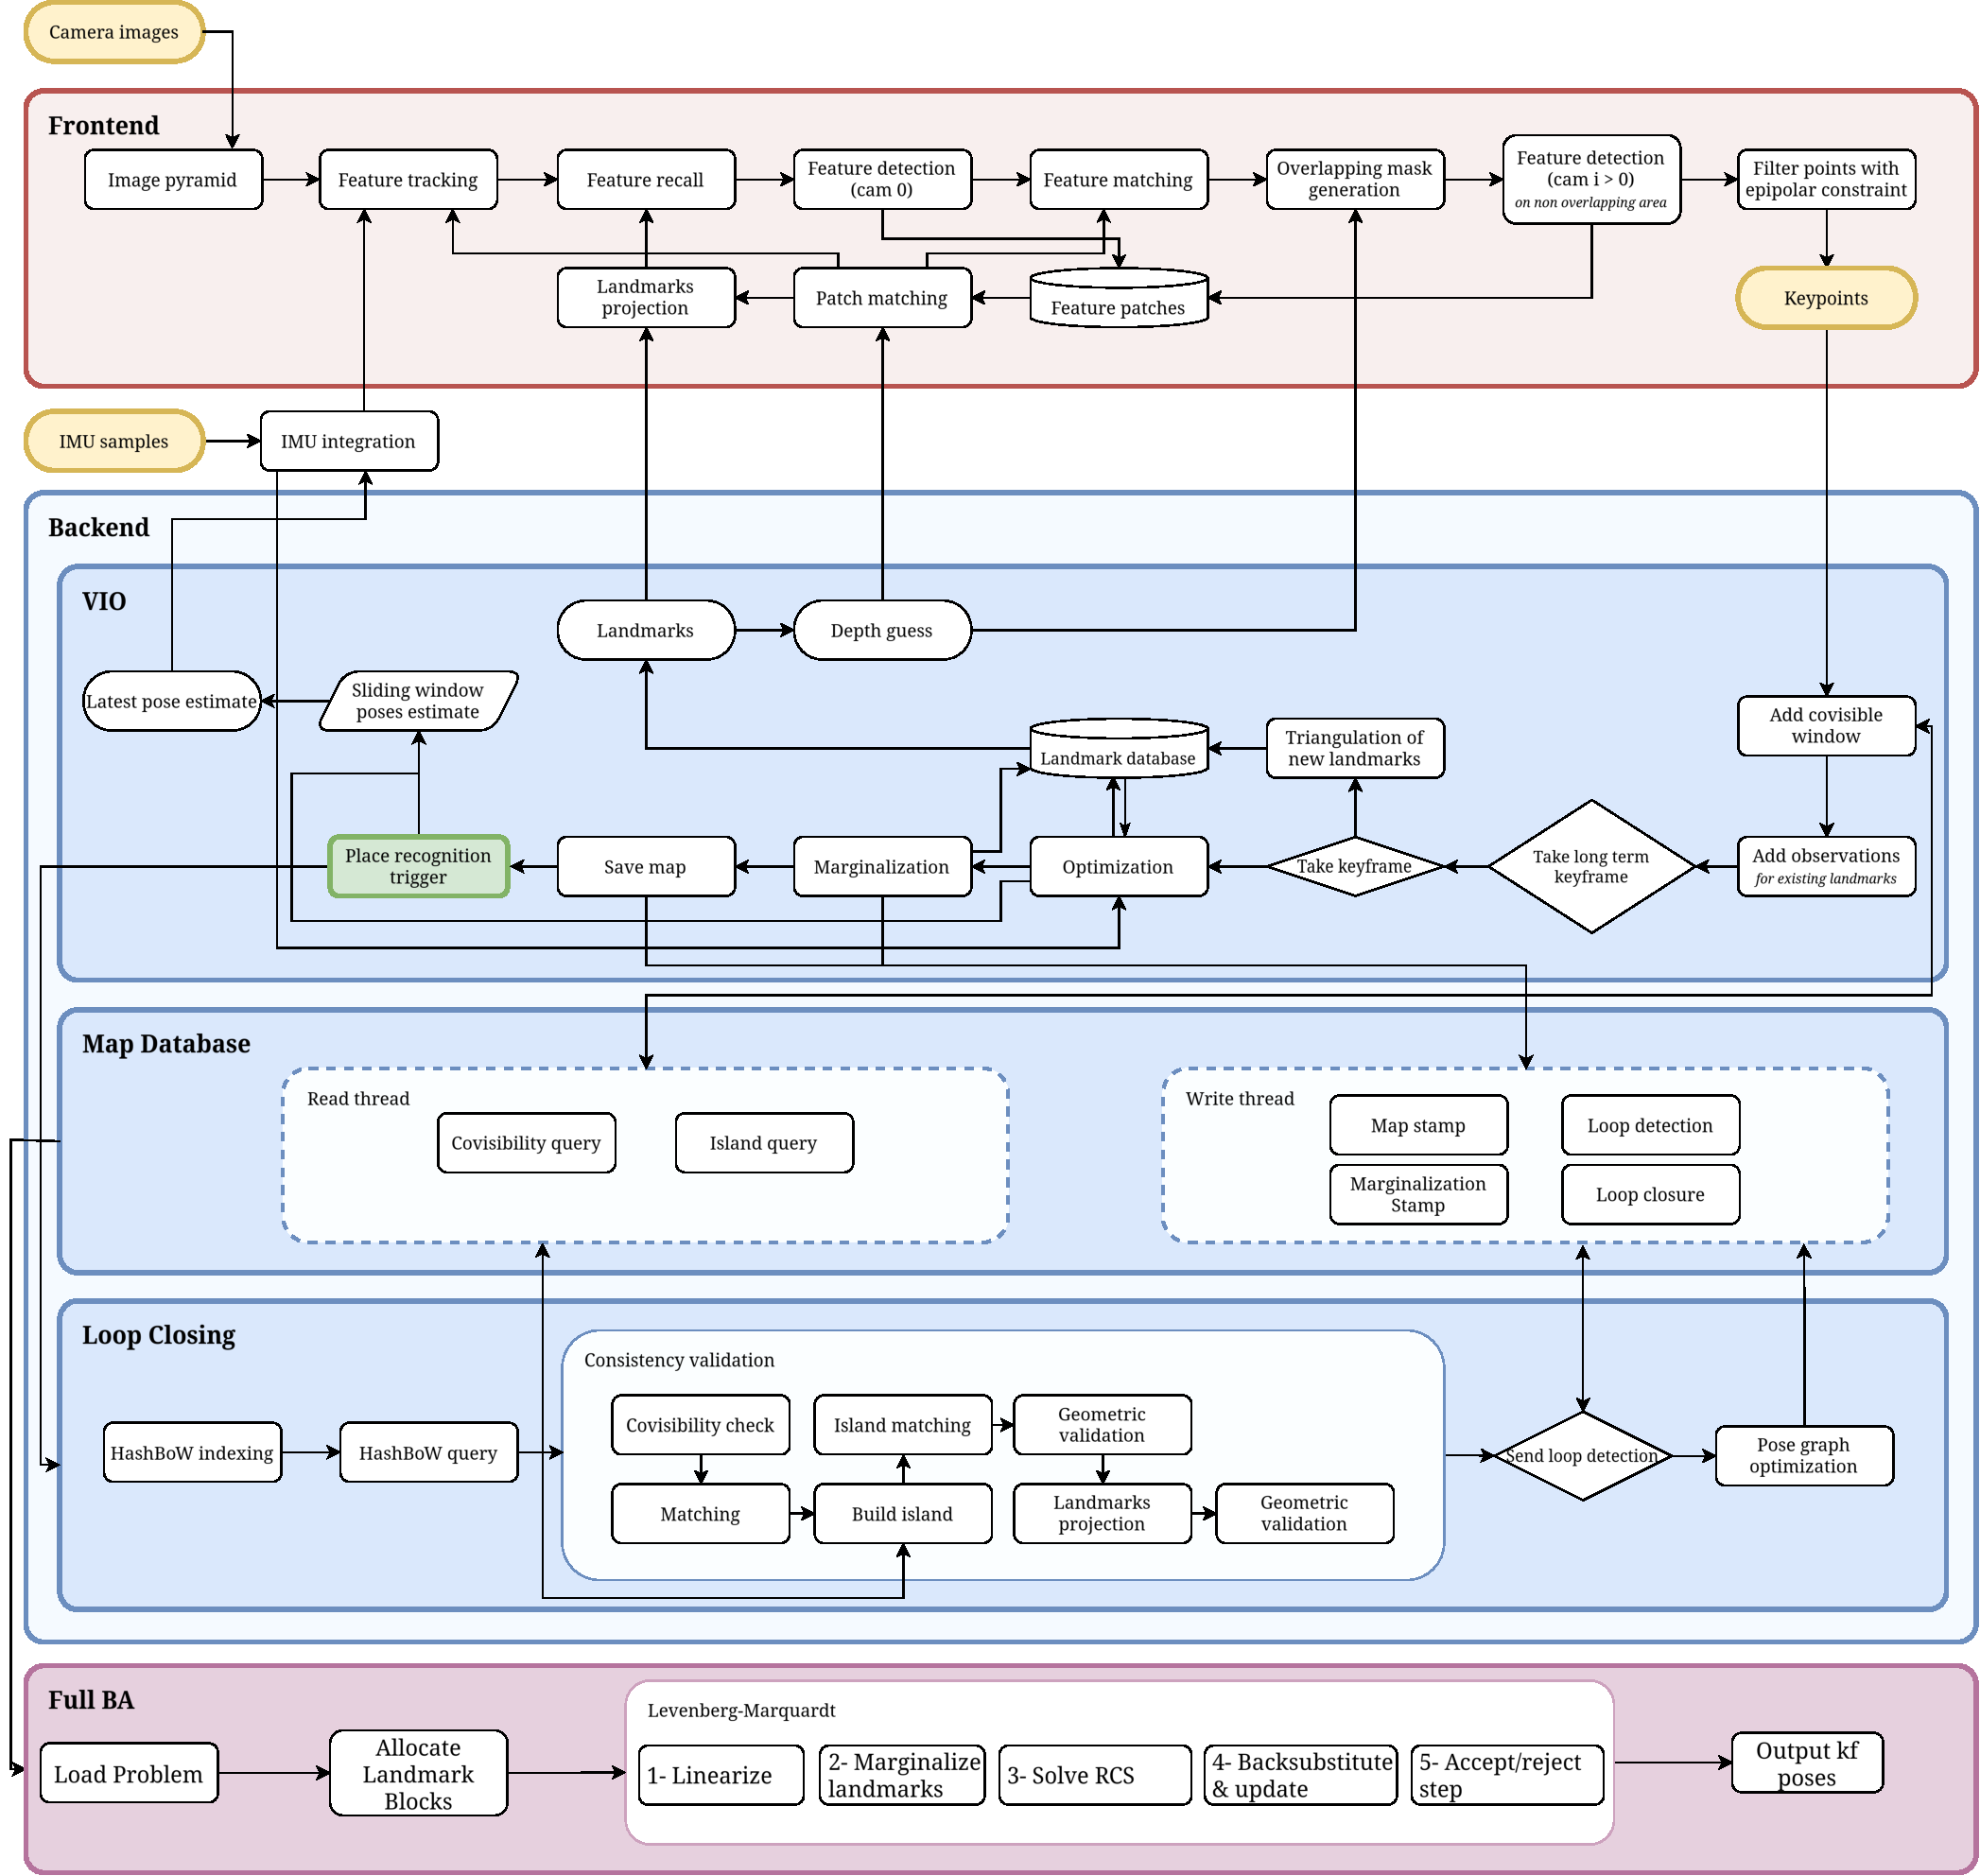
\includegraphics[width=1\linewidth]{images/system-arch.pdf}
    \caption{Arquitectura del sistema VI-SLAM propuesto. Se incorporan los componentes \texttt{Loop Closing} y \texttt{RootBA Full}, y se extiende \texttt{Map Database}.}
    \label{fig:system-pipeline}
\end{figure}

En este trabajo presentamos una serie de funcionalidades en Basalt (ver Figura \ref{fig:system-pipeline}), que lo transforman en un sistema VI-SLAM con precisión comparable al estado del arte. Tomamos como punto de partida BasaltXR \cite{zanotti2024basaltxr}, que a su vez extiende la versión de Basalt utilizada en \cite{demayo2025monadoslamdataset}.
Las mejoras están diseñadas para aumentar la precisión del sistema mediante el uso de información del mapa, manteniendo la eficiencia característica de Basalt.

\subsection{Mapa Persistente}

En primer lugar, se enriqueció la clase \texttt{MapDatabase} para soportar más operaciones y habilitar la utilización del mapa de manera más inteligente. Se implementó una estructura llamada \texttt{CovibilityGraph} que contiene grafos que acumulan información de interés y se mantienen actualizados en todo momento, inspirada en el \textit{Essential Graph}, introducido en \cite{campos2021orbslam3}. Entre ellos: un grafo pesado de covisibilidad, que se usa para resolver consultas del back-end y del componente de \texttt{LoopClosing} para la detección de ciclos; un árbol de expansión, que mantiene a todos los keyframes conectados y es utilizado al realizar Pose Graph Optimization; un grafo no dirigido que almacena aristas entre keyframes involucrados en cierres de ciclos; un grafo no dirigido, que guarda aristas que tengan un peso alto en el grafo de covisibilidad, y se utiliza en Pose Graph Optimization.

Además, se introdujo un mecanismo de culling de keyframes con dos estrategias, que evitan introducir keyframes redundantes al mapa, y que este crezca de manera indefinida: (1) Cada vez que el back-end marginaliza un keyframe, se verifica la redundancia de la información que aporta al mapa. Si más de un 90\% de sus observaciones corresponden a landmarks que ya son observados por, al menos, otros 3 keyframes del mapa, se elimina. (2) Cada vez que el mapa supera un total de 1500 keyframes, se eliminan 30 de ellos. Para seleccionarlos, se utiliza una suma pesada de diferentes heurísticas como función de scoring. Este puntaje penaliza a los keyframes de mala calidad, o que resulten reemplazables teniendo en cuenta el grafo de covisibilidad. Cada vez que se elimina un keyframe, en ambas estrategias, también se remueven todos los landmarks que este hosteaba.

\subsection{Detección y Cierre de Ciclos}
Si bien BasaltXR extiende a Basalt para funcionar como un sistema de VI-SLAM, solo soporta asociaciones de datos a corto y mediano plazo. Para obtener un sistema más completo, se introduce la asociación de datos a largo plazo, mediante el cierre de ciclos y la fusión de mapa.

Se introdujo el componente \texttt{LoopClosing} en un thread separado que recibe las imágenes de cada keyframe y los keypoints detectados en ellas, de manera online.

Para la detección de candidatos a cierre de ciclo se emplea HashBoW \cite{hashbow2024stricker}, el esquema de bag of words más rápido entre sus alternativas. Para cada keyframe, se computan descriptores ORB~\cite{rublee2011orb} sobre los keypoints detectados y se construye el correspondiente vector de bag of words, con el que se consulta la base de datos.
Dado que estos métodos suelen producir un gran número de falsos positivos, los candidatos obtenidos pasan por una serie de validaciones de consistencia. Entre ellas, se realiza matching a fuerza bruta y reproyecciones de landmarks para establecer correspondencias 3D--2D. Finalmente se ejecuta una validación geométrica mediante gP3P \cite{kneip2013gp3p} con la librería OpenGV \cite{kneip2022opengv}.

Al detectarse un ciclo, se notifica al mapa persistente. En función del drift estimado, el mapa decide entre dos acciones: si es menor a 10 cm, simplemente fusiona los landmarks validados como inliers; en caso contrario, se ejecuta una optimización global y luego la fusión. Para ello, el mapa genera una copia de las poses de todos los keyframes y la envía al thread de loop closure junto con el árbol de expansión, las aristas de alta covisibilidad y de ciclos previos. Con esta información, se construye un grafo de poses y se optimiza mediante Pose Graph Optimization. Finalmente, el thread de loop closing devuelve las poses corregidas al mapa persistente para su sincronización.

\subsection{Optimización Global}
A partir del mapa resultante del sistema propuesto, así como realizan algunos sistemas VI-SLAM del estado del arte \cite{campos2021orbslam3} \cite{leutenegger2022okvis2}, es posible ejecutar una optimización global de bundle adjustment, de manera offline. El obtetivo es refinar las poses de los keyframes y posiciones de landmarks de manera conjunta.

Para ello, se adaptó el método de Square Root Bundle Adjustment a gran escala (RootBA) propuesto en \cite{demmelBasaltSquareRoot2021a}, originalmente diseñado para SfM.

El estado en la implementación de RootBA\footnote{\href{https://github.com/nikolausdemmel/rootba}{github.com/nikolausdemmel/rootba}}
se divide en una parte de poses $x_p$, que a su vez se subdivide en parámetros extrínsecos $x_c$ (las poses ${T_i \in SE(3)}$) e intrínsecos $x_i$ (distancia focal $f_i$ y distorsión radial $k_1^i, k_2^i$) para cada una de las $n_p$ cámaras, y una parte de landmarks $x_l$ con las coordenadas 3D de los $n_l$ puntos. El problema consiste en minimizar la ecuación de energía:
\begin{equation}
E(x_c, x_i, x_l) = \sum_{i}\sum_{j \in \mathcal{O}(i)} |r_{ij}(x_c, x_i, x_l)|^2,
\label{eq:ba_energy}
\end{equation}
donde $j \in \mathcal{O}(i)$ indica que el landmark $j$ es observado en el frame $i$. El vector de estado completo tiene longitud $9n_p + 3n_l$. La información relacionada a los jacobianos y residuales de cada landmark se condensa en matrices llamadas \textit{Landmark Blocks}.

\textbf{Eliminación de parámetros intrínsecos.} En SfM, $x_i$ es desconocido pues las imágenes pueden provenir de cámaras distintas. En SLAM las calibraciones suelen ser conocidas y fijas, por lo que optimizar $x_i$ es contraproducente: el optimizador podría absorber errores de pose modificando la calibración en lugar de corregir $x_c$. La solución es eliminar $x_i$ del estado, reduciendo la ecuación de energía a $E(x_c, x_l)$ y la dimensión por cámara de $d_p = 9$ a $d_p = 6$. Las columnas correspondientes a $x_i$ se suprimen en los Landmark Blocks sin alterar la estructura de la factorización QR, y evitando el cálculo de los jacobianos con respecto a los parámetros intrínsecos.

\textbf{Optimización de poses de rig.} En un sistema SLAM multicámara basado en keyframes, cada uno de ellos es un rig compuesto por múltiples cámaras $c_k$ con $k \in \{0, 1, \ldots \}$. La transformación de cada cámara $c_k$ al body, $T_{c_k b} \in SE(3)$, es conocida (dada por la calibración extrínseca) y constante a lo largo de todos los keyframes. La pose de cada cámara se obtiene entonces como $T_{c_k} = T_{c_k b}\cdot T_b$, donde $T_b$ es la pose del body. En lugar de almacenar en $x_c$ una pose por cámara por keyframe, lo que podría romper esta restricción de rigidez, se parametriza el estado con las poses del body $x_b$. Esto requiere reparametrizar los Jacobianos: dado que $\Delta x_{c_k} = \mathrm{Ad}_{T_{c_k b}} \Delta x_b$, la regla de la cadena da
\begin{equation}
\frac{\partial r}{\partial \Delta x_b} = \frac{\partial r}{\partial \Delta x_{c_k}} \cdot \frac{\partial \Delta x_{c_k}}{\partial \Delta x_b} = \frac{\partial r}{\partial \Delta x_{c_k}}\cdot \mathrm{Ad}_{T_{c_k b}}.
\end{equation}
Como consecuencia, un mismo Landmark Block puede acumular observaciones de distintas cámaras del rig en una única columna correspondiente a una variable $x_b$.

La Figura~\ref{fig:landmark_block} ilustra el efecto conjunto de ambas modificaciones sobre la estructura de un Landmark Block.

\begin{figure}[!htbp]
    \centering
    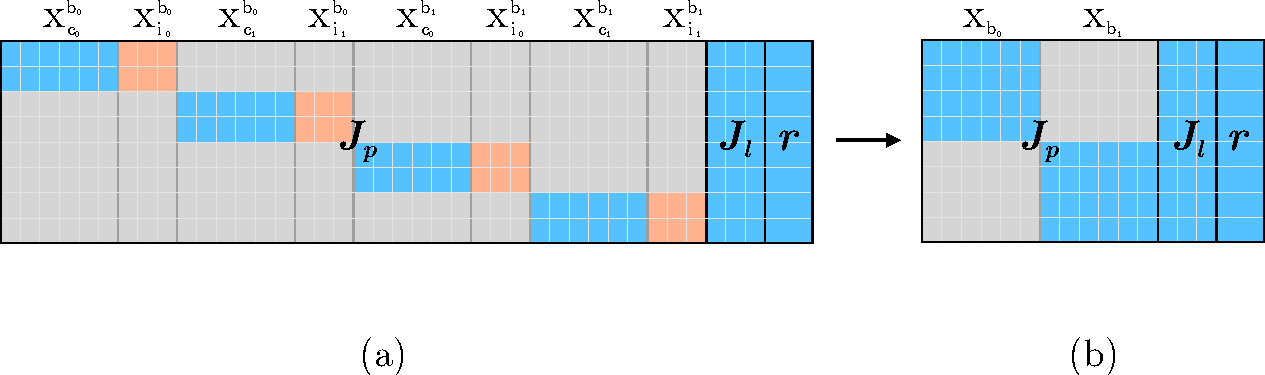
\includegraphics[width=\linewidth]{images/rootba-mod.pdf}
    \caption{Estructura de un Landmark Block. (a)~RootBA original: estado por cámara de dimensión $d_p = 9$, incluyendo parámetros intrínsecos $x_i$ en naranja. (b)~Versión adaptada: $d_p = 6$ (intrínsecos eliminados), con observaciones de múltiples cámaras del rig acumuladas en la variable de body $x_b$.}
    \label{fig:landmark_block}
\end{figure}
